\documentclass[twoside,a4paper,12pt]{article}

\usepackage{EthischeFragenBeimAutomatisiertenFahren}

\begin{document}

\thispagestyle{empty}
\begin{center}
	
\includegraphics[scale=1]{resources/fernunisignet-sw}
\end{center}
\vskip 4cm
\begin{center}
	{\Large Seminararbeit 1902 WS 2018/19\par}
	\vskip 2.5cm
	{\textbf{\Large Ethische Fragen} \par}    
	\vskip 0.2cm	
	{\textbf{\Large beim automatisierten Fahren} \par}    
	\vskip 1cm
	{\Large Nikolai Kabiolskij\\Christian Oevermann \par}
	\vskip 4.5 cm
	\Large Januar 2019
\end{center}
\vspace*{\stretch{1}}
\FUiH\\
Fakultät für Mathematik und Informatik\\
Lehrgebiet Kooperative Systeme\\
Betreut von apl. Prof. Dr. Christian Icking und Dr. Lihong Ma\\
  
\newpage
\shipout\hbox{}
\newpage

\frontmatter

\section{Einleitung} \label{Einleitung}
Schon seit jeher wollen die Menschen sich fortbewegen können und ihren Aktionsradius erweitern und haben Ihre Mobilität zunehmend ausgebaut. Mit der rasanten
Entwicklung von Technologien und der zunehmenden Digitalisierung aller Lebensbereiche entstehen neue Möglichkeiten, die für die Mobilität der Zukunft eingesetzt 
werden können und sollen. Das Thema dieser Ausarbeitung ist das \textit{hochautomatisierte} bzw. das \textit{autonome} Fahren, konkret werden dabei aufkommende
ethischen Fragen erläutert und hinsichtlich ihrer möglichen Antworten kritisch beleuchtet. \\ 

Auch wenn das autonome Fahren sicher scheint, wenn hierfür nur ausgereifte technische Systeme eingesetzt werden, so ist doch die Möglichkeit von Unfällen gegeben ---
mit der Folge von Sachschäden, Körperverletzungen oder Tod von Verkehrsteilnehmern oder auch Unbeteiligten. Beispielsweise kann es in Unfallsituationen zu der
Notwendigkeit kommen, \textit{Dilemma-Entscheidungen} treffen zu müssen, Entscheidungen also, bei denen es auf jeden Fall zu Personen- oder Sachschäden kommt
und bei denen keine der möglichen Varianten ethisch vollkommen \glqq richtig\grqq\ ist. Häufig wird die Entscheidung in einer gegebenen Situation auch von Mensch zu
Mensch unterschiedlich ausfallen. \\ 

Um all die ethischen Fragen rund um automatisiertes und autonomes Fahren zu beantworten oder zumindest aufzuwerfen, wurde von dem damaligen Bundesverkehrsminister Dobrindt eine Expertenrunde unter Leitung des ehemaligen Bundesverfassungsrichter Udo Di Fabio einberufen. Die \textit{Ethik-Kommission
des Bundesministeriums für Verkehr und digitale Infrastruktur (BMVI)} setzte sich aus vierzehn Wissenschaftlern und Experten aus den Fachrichtungen Ethik, Recht und Technik zusammen.~\cite{bmvi1} Aufgabe der Kommission war es, grundlegende ethische Leitlinien für die Entwicklung von autonom fahrenden Systemen zu
erarbeiten. Das Ergebnis der fünf Sitzungen der Kommission ist ein Manifest mit zwanzig ethischen Grundregeln für den automatisierten, autonomen und vernetzten Fahrzeugverkehr. Diese Regeln werden in der folgenden Ausarbeitung zitiert, erläutert und auf ihre Anwendbarkeit hin hinterfragt. 

\newpage

\tableofcontents

\vspace*{\stretch{1}}

\listoffigures

\newpage

\mainmatter

\cleardoublepage
\section{Vorstellung und Kommentierung der Ethik-Regeln} \label{VorstellungUndKommentierungDerEthikRegeln}

Im nachfolgenden Hauptteil dieser Ausarbeitung werden jeweils die von der Kommission formulierten ethischen Regeln zitiert und im Anschluss einer kritischen 
Würdigung hinsichtlich ihrer technischen Implementierbarkeit und der Kompatibilität mit heutigen gesellschaftlichen Normen unterzogen. 
Diese fällt i.\,d.\,R. wegen der gebotenen Kürze knapp aus und ist selbstverständlich
stark von der subjektiven Einschätzung der Autoren geprägt. Naturgemäß wirft sie eher weiterführende Fragen auf, als dass sie Antworten lieferte.\\

Bevor wir uns den Regeln im Einzelnen zuwenden, wollen wir kurz die Automatisierungsgrade beim automatisierten Fahren klären. Der Verband der 
Automobilindustrie (VDA)~\cite{vda} systematisiert diese so wie in \autoref{figure:Automatisierungsgrade} dargestellt.\\

\begin{figure}[H]
\centering
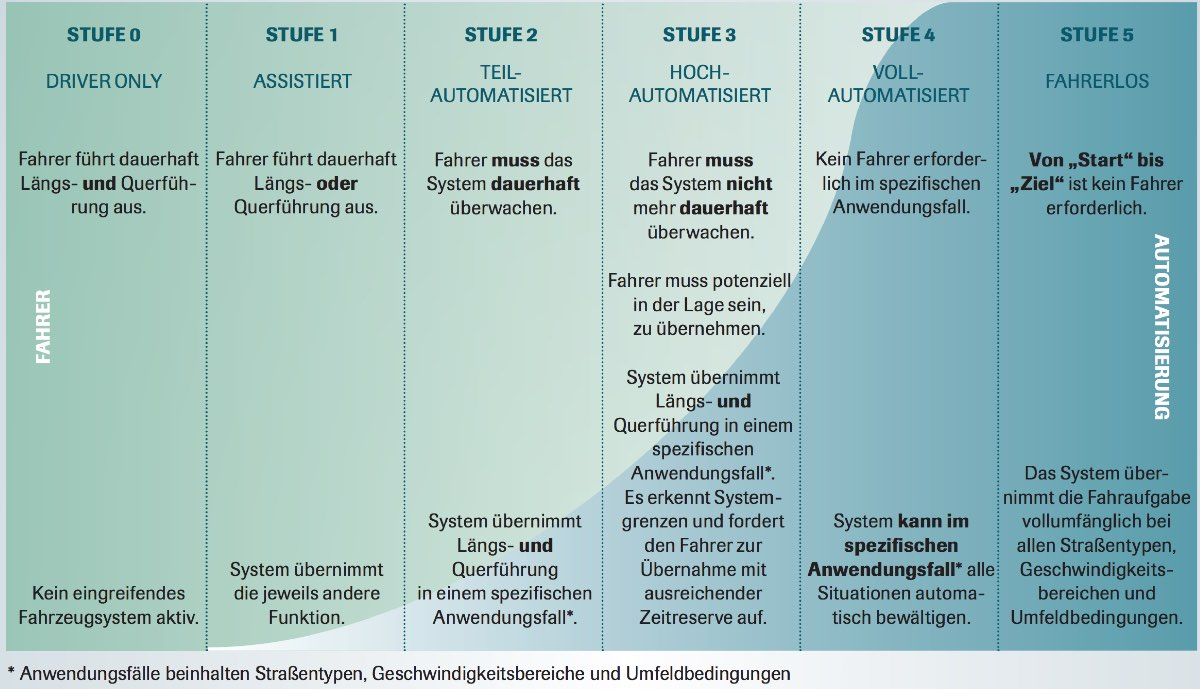
\includegraphics[width=11cm]{resources/uebersicht-stufen-der-automatisierung.jpg}
\caption[Automatisierungsgrade des automatisierten Fahrens]{Automatisierungsgrade des automatisierten Fahrens~\cite{vda}}
\label{figure:Automatisierungsgrade}
\end{figure}

Die folgenden Regeln beziehen sich vor allem auf die Stufen 4 und 5, also auf das \textit{vollautomatisierte} und das \textit{fahrerlose} Fahren.
Prinzipiell gelten sie natürlich für sämtliche Automatisierungsgrade.\\

\subsection{Primärziel Sicherheit} \label{PrimaerzielSicherheit}

\begin{quote}
\glqq
Teil- und vollautomatisierte Verkehrssysteme dienen zuerst der Verbesserung der Sicherheit aller Beteiligten im Straßenverkehr. 
Daneben geht es um die Steigerung von Mobilitätschancen und die Ermöglichung weiterer Vorteile. Die technische Entwicklung 
gehorcht dem Prinzip der Privatautonomie im Sinne eigenverantwortlicher Handlungsfreiheit.\grqq\mbox{~\cite[S. 10]{ek}}
\end{quote}

Autonom fahrende und vernetzte Fahrzeuge sind nur dann ethisch vertretbar,
wenn sie die Unfallwahrscheinlichkeit gegenüber menschlichen Fahrern verringern und zum allgemeinem Verkehrsfluss positiv beitragen.
Weiterhin müssen die autonomen Fahrzeuge so konzipiert werden, dass sie auch auf andere Verkehrsteilnehmer wie Fußgänger und 
Radfahrer, aber auch nicht autonom fahrende Fahrzeuge vorbereitet sind und mit deren Fehlern rechnen. Die Systeme müssen bereit 
sein, auch auf nicht vorhersehbare Situationen zu reagieren, um das Risiko von Unfällen zu minimieren. Hier 
geht Sicherheit klar vor Komfort, d.\,h. nicht mehr selbst fahren zu müssen und sich derweil anderen Dingen zu widmen.
Darüber hinaus könnten
vernetzte und autonome Fahrzeuge den Verkehr flüssiger gestalten und insgesamt das Fahren in dicht bewohnten Städten angenehmer machen. 
Dabei ist durchaus denkbar, dass diese Systeme im Gegensatz zu menschlichen Fahrern den Raum auf der Straße optimal ausnutzen und weniger Staus verursachen.
Die Kommission weist darauf hin, dass trotz der vielen Chancen und Vorteile des autonomen Fahrens insbesondere die Risikoaspekte im gemischten Verkehr neu 
betrachtet und Haftungsfragen neu beantwortet werden müssen. Außerdem stellt die Kommission in derselben Leitlinie klar, dass potentielle Nutzer eigenverantwortlich selbst entscheiden dürfen, ob und wie sie das autonome Fahren verwenden möchten. Solche persönlichen Entscheidungen dürfen keineswegs eingeschränkt oder gar
aufgezwungen werden.\\

\subsection{Vorrang des Schutzes von Menschen} \label{VorrangDesSchutzesVonMenschen}

\begin{quote}
\glqq
Der Schutz von Menschen hat Vorrang vor allen anderen Nützlichkeitserwägungen. Ziel
ist die Verringerung von Schäden bis hin zur vollständigen Vermeidung. Die Zulassung
von automatisierten Systemen ist nur vertretbar, wenn sie im Vergleich zu menschlichen
Fahrleistungen zumindest eine Verminderung von Schäden im Sinne einer positiven Risikobilanz verspricht.\grqq\mbox{~\cite[S. 10]{ek}}
\end{quote}

Die Entwicklung von Systemen zum autonomen Fahren sollte stets das Ziel, menschliches Leben zu schützen, 
als primäres Ziel im Auge behalten. Alle weiteren bereits angesprochenen Ziele wie Komfort, verbesserter Verkehrsfluss o.ä. sind allesamt sekundär 
und dürfen keineswegs vorangestellt werden. Diese Ansätze müssen bereits im Kern der Implementierung berücksichtigt und stets weiterverfolgt werden. Nur unter 
diesen Umständen ist es ethisch vertretbar, solche Systeme überhaupt zuzulassen und massenhaft zu betreiben. Der Schutz menschlichen Lebens ist ein sehr umfassendes Thema und wurde natürlich von der Kommission viel breiter diskutiert. Weiterführende Gedanken zu diesem Thema finden sich daher in einem \hyperlink{target1}{weiteren Kapitel} dieser Arbeit.\\

\subsection{Gewährleistungsverantwortung der öffentlichen Hand} \label{GewaehrleistungsverantwortungDerOeffentlichenHand}

\begin{quote}
\glqq
Die Gewährleistungsverantwortung für die Einführung und Zulassung automatisierter
und vernetzter Systeme im öffentlichen Verkehrsraum obliegt der öffentlichen Hand.
Fahrsysteme bedürfen deshalb der behördlichen Zulassung und Kontrolle. Die Vermeidung von Unfällen ist Leitbild, wobei technisch 
unvermeidbare Restrisiken einer Einführung des automatisierten Fahrens bei Vorliegen einer grundsätzlich positiven Risikobilanz
nicht entgegenstehen.\grqq\mbox{~\cite[S. 10]{ek}}
\end{quote}

So wie heute alle Fahrzeuge in Deutschland einer Haupt- und Abgasuntersuchung unterzogen werden müssen, sollten ähnliche Zulassungs-Maßnahmen für autonom
fahrende Fahrzeuge geschaffen werden. Dabei gilt es zu beachten, dass in der heutigen globalisierten Welt zunächst verbindliche Normen geschaffen werden müssen was  die Definition eines sicheren, autonomen Fahrzeuga allgemein betrifft. Die Ausarbeitung solcher Normen muss von den Regierungen einzelner Staaten der EU und möglichst der ganzen restlichen Welt vorgenommen werden. Dabei muss bedacht werden, dass die Vereinheitlichung aller Normen ebenso erfolgen muss. So wie einst das
ECE-Prüfzeichen geschaffen wurde, wäre eine einheitliche europäische Kennzeichnung von zugelassenen Systemen denkbar. Dabei macht die Kommission selbst einen wichtigen Schritt und formuliert zunächst ein Regelwerk mit ethischen Regeln für die Umsetzung von autonomen Systemen. Es scheint nur plausibel, dass hier das Autoland Deutschland eine Vorreiterrolle einnimmt.\\

\subsection{Entscheidungsfreiheit des Einzelnen} \label{EntscheidungsfreiheitDesEinzelnen}

\begin{quote}
\glqq
%% 2.4
Die eigenverantwortliche Entscheidung des Menschen ist Ausdruck einer Gesellschaft, in
der der einzelne Mensch mit seinem Entfaltungsanspruch und seiner Schutzbedürftigkeit
im Zentrum steht. Jede staatliche und politische Ordnungsentscheidung dient deshalb
der freien Entfaltung und dem Schutz des Menschen. In einer freien Gesellschaft erfolgt
die gesetzliche Gestaltung von Technik so, dass ein Maximum persönlicher Entscheidungsfreiheit in einer allgemeinen 
Entfaltungsordnung mit der Freiheit anderer und ihrer
Sicherheit zum Ausgleich gelangt.\grqq\mbox{~\cite[S. 10]{ek}}
\end{quote}

Hiermit möchte die Kommission zum Ausdruck bringen, dass es niemals der Weg sein kann, den Menschen das autonome Fahren aufzuzwingen und selbstständiges
manuelles Fahren zu verbieten. Solch ein Verbot würde die Handlungsfreiheit eines Fahrzeugführers unzulässig einschränken. Daher müssen alle Regeln, die die
Kommission präsentiert, so verstanden werden, dass sie nicht zwingend dazu führen dürfen, dass künftig ausschließlich autonom gefahren werden darf. Die erhöhte Sicherheit im Straßenverkehr überwiegt als anzustrebendes Gut nicht die Freiheit aller Individuen, selbst zu entscheiden, wie sie sich fortbewegen möchten.\\

\subsection{Unfallvermeidung} \label{Unfallvermeidung}

\begin{quote}
\glqq
%% 2.5
Die automatisierte und vernetzte Technik sollte Unfälle so gut wie praktisch möglich vermeiden. Die Technik muss nach 
ihrem jeweiligen Stand so ausgelegt sein, dass kritische
Situationen gar nicht erst entstehen, dazu gehören auch Dilemma-Situationen, also eine
Lage, in der ein automatisiertes Fahrzeug vor der \glqq Entscheidung\grqq\ steht, eines von zwei
nicht abwägungsfähigen Übeln notwendig verwirklichen zu müssen. Dabei sollte das gesamte Spektrum technischer 
Möglichkeiten --- etwa von der Einschränkung des Anwendungsbereichs auf kontrollierbare Verkehrsumgebungen, 
Fahrzeugsensorik und Bremsleistungen, Signale für gefährdete Personen bis hin zu einer Gefahrenprävention mittels
einer \glqq intelligenten\grqq\ Straßen-Infrastruktur --- genutzt und kontinuierlich weiterentwickelt
werden. Die erhebliche Steigerung der Verkehrssicherheit ist Entwicklungs- und Regulierungsziel, und zwar bereits in der 
Auslegung und Programmierung der Fahrzeuge zu defensivem und vorausschauendem, schwächere Verkehrsteilnehmer (\glqq Vulnerable Road
Users\grqq) schonendem Fahren.\grqq\mbox{~\cite[S. 10]{ek}}
\end{quote}

Mit diesem Satz möchte die Kommission die Fahrzeughersteller dazu verpflichten, autonome Fahrsysteme so zu entwickeln, dass Gefahrensituationen oder gar Unfälle
möglichst gar nicht erst entstehen. Es müssen alle vorhandenen technischen Möglichkeiten ausgenutzt werden, um die Sicherheit von schwächeren Verkehrsteilnehmern wie
Radfahrern oder Fußgängern zu gewährleisten und weitgehend unfallfreies Fahren zu ermöglichen. So wie derzeit Fahrschüler die Regeln für defensives und
vorausschauendes Fahren in der Fahrschule beigebracht bekommen, müssen dieselben Regeln auch für automatisierte oder autonome Fahrzeuge gelten. Hier werden die Hersteller bzw. Systembetreiber in die Pflicht genommen.\\ 

Es gibt aber auch Beispiele, bei denen die Menschen notgedrungen Straßenverkehrsregeln brechen. So wird ein in der zweiten Reihe mit Warnblinker stehendes Auto
möglicherweise ein autonomes Fahrzeug komplett zum Stehen bringen, weil das autonome Auto eine durchgezogene Mittellinie nicht überschreiten darf.~\cite{zeit1} Jeder Fahrer würde in dieser Situation wohl ohne Bedenken die Fahrstreifenbegrenzung überqueren, autonome Fahrzeuge höchstwahrscheinlich hingegen nicht. Man könnte das
Beispiel ausweiten und sich vorstellen, dass sich in solchen Fällen viele autonome Fahrzeuge hintereinander stellen werden und die komplette Straße ungewollt blockieren. Es wird vorerst schwierig bleiben, derartige Ausnahmesituationen adäquat abzufangen und technisch sauber zu implementieren. Ob man das Auto dazu bewegt, die
Verkehrsregeln zu umgehen, um diese Situation zu bewältigen, oder zum Beispiel die Steuerung an den menschlichen Fahrer übergibt, lässt die Ethik-Kommission offen.\\ 

\subsection{Abwägungen zur Einsatzpflicht} \label{AbwaegungenZurEinsatzpflicht}

%%2.6
\begin{quote}
\glqq
Die Einführung höherer automatisierter Fahrsysteme insbesondere mit der Möglichkeit
automatisierter Kollisionsvermeidung kann gesellschaftlich und ethisch geboten sein,
wenn damit vorhandene Potentiale der Schadensminderung genutzt werden können.
Umgekehrt ist eine gesetzlich auferlegte Pflicht zur Nutzung vollautomatisierter Verkehrssysteme oder die Herbeiführung 
einer praktischen Unentrinnbarkeit ethisch bedenklich, wenn damit die Unterwerfung unter technische Imperative verbunden 
ist (Verbot der Degradierung des Subjekts zum bloßen Netzwerkelement).\grqq\mbox{~\cite[S. 11]{ek}}
\end{quote}

Wie vorher bereits erwähnt schließt die Kommission den Zwang zum autonomen Fahren ausdrücklich aus. Gleichzeitig ist es natürlich ethisch vertretbar, die Menschen dazu zu bringen, autonome Fahrzeuge verstärkt zu nutzen. Diese Empfehlung wird von der Ethik-Kommission ausgesprochen, solange gewährleistet ist, dass dadurch eine allgemeine Schadensminderung gegenüber manuellem Fahren erreicht werden kann. \\

In vielen Fällen können weitere, für die Industrie, Hersteller oder Betreiber nützliche Nebeneffekte entstehen. Sollten in Fahrzeugen diverse Computer eingesetzt werden, können verschiedenste Daten anfallen und ausgewertet werden. In diesem Zusammenhang möchte die Kommission auf die Datensparsamkeit und Datenvermeidung gemäß dem Bundesdatenschutzgesetz hinweisen und der Datensammelei eine klare Absage erteilen. Nach Ansicht der Mitglieder der Kommission ist es ethisch zumindest bedenklich, die Fahrzeugführer bzw. Passagiere lediglich zu einer lukrativen Datenquelle werden zu lassen.\\

\subsection{Priorität des Schutzes menschlichen Lebens} \label{PrioritäDesSchutzesMenschlichenLebens}

\begin{quote}
\glqq
\hypertarget{target1}
In Gefahrensituationen, die sich bei aller technischen Vorsorge als unvermeidbar erweisen, besitzt der Schutz menschlichen 
Lebens in einer Rechtsgüterabwägung höchste Priorität. Die Programmierung ist deshalb im Rahmen des technisch Machbaren 
so anzulegen, im Konflikt Tier- oder Sachschäden in Kauf zu nehmen, wenn dadurch Personenschäden vermeidbar sind.\grqq\mbox{~\cite[S. 11]{ek}}
\end{quote}

In Gefahrensituationen genießt der Schutz des menschlichen Lebens die höchste Priorität. So bedeutet, dass im Falle eines Unfalls Sachschäden in Kauf genommen werden
müssen um Menschenleben zu retten. Diese Aussage scheint auf den ersten Blick ethisch einleuchtend zu sein, jedoch können dabei Nachfolgekomplikationen auftreten. So nennt die Kommission ein Beispiel, in dem folgende Situation beschrieben wird:

\begin{quote}
\dots die Folge eines Sachschadens [könnte] das Auslaufen eines Tanklasters oder auch der Zusammenbruch des Stromnetzes einer Metropolregion sein \dots
\mbox{~\cite[S.17]{ek}}
\end{quote}

Das Beispiel zeigt, dass manche Sachschäden eventuell enorme Auswirkungen mit sich bringen, die unter Umständen zu weiteren Personenschäden führen. Daher führt die
Anwendung des Leitsatzes \glqq Sachschäden gehen vor Personenschäden\grqq\ nicht zwangsläufig zum besten Ergebnis. In diesem Punkt wäre eine mögliche Folgenabschätzung von Sachschäden erforderlich, eine Aufgabe, die ein IT-System (zumindest derzeit) deutlich überfordern dürfte.
Es muss hier aber auch erwähnt werden, dass selbst Menschen niemals in der Lage sind, sich alle möglichen Ausgänge eines Unfalls in kürzesten Zeit zu vergegenwärtigen, daher werden sie meist intuitiv entscheiden. Fazit bleibt: Eine korrekte Behandlung aller Eventualitäten dürfte vorerst technisch schwer umsetzbar sein.\\

%% gelesen
\subsection{Keine Normierbarkeit dilemmatischer Entscheidungen} \label{NichtNormierbarkeitDilemmatischerEntscheidungen}
%% 2.8

\begin{quote}
\glqq
Echte dilemmatische Entscheidungen, wie die Entscheidung Leben gegen Leben sind von
der konkreten tatsächlichen Situation unter Einschluss \glqq unberechenbarer\grqq\ Verhaltensweisen Betroffener abhängig. 
Sie sind deshalb nicht eindeutig normierbar und auch nicht
ethisch zweifelsfrei programmierbar. Technische Systeme müssen auf Unfallvermeidung
ausgelegt werden, sind aber auf eine komplexe oder intuitive Unfallfolgenabschätzung
nicht so normierbar, dass sie die Entscheidung eines sittlich urteilsfähigen, verantwortlichen Fahrzeugführers ersetzen 
oder vorwegnehmen könnten. Ein menschlicher Fahrer
würde sich zwar rechtswidrig verhalten, wenn er im Notstand einen Menschen tötet, um
einen oder mehrere andere Menschen zu retten, aber er würde nicht notwendig schuldhaft handeln. Derartige in der Rückschau 
angestellte und besondere Umstände würdigende Urteile des Rechts lassen sich nicht ohne weiteres in abstrakt-generelle 
Ex-Ante Beurteilungen und damit auch nicht in entsprechende Programmierungen umwandeln.
Es wäre gerade deshalb wünschenswert, durch eine unabhängige öffentliche Einrichtung
(etwa einer Bundesstelle für Unfalluntersuchung automatisierter Verkehrssysteme oder
eines Bundesamtes für Sicherheit im automatisierten und vernetzten Verkehr) Erfahrungen systematisch zu verarbeiten.\grqq\mbox{~\cite[S. 11]{ek}}
\end{quote}

Mit diesem Regelsatz möchte die Ethik-Kommission auf eine der wichtigsten und gleichzeitig am schwierigsten zu beantwortenden Fragen eingehen. Tatsächlich sind dilemmatische Entscheidungen auch von Menschen nur sehr schwer zu treffen. Zudem ist davon auszugehen, dass alle möglichen Handlungsweise rechtswidrig sein können.
Da jedoch autonome Systeme zwingend zu einer Entscheidung kommen müssen, stellt sich die Frage der Implementierung. Falls die Maschine nicht entscheiden kann, muss
dies eine Person für sie übernehmen. Gegenwärtig ist man als Fahrer selbst für seine Handlungen am Steuer verantwortlich. Sollen jedoch autonome Systeme übernehmen,
wäre dies nicht mehr der Fall. Dabei sind verschiedene Szenarien denkbar: die Entscheidung wird vom Produkthersteller oder von einer zuständigen Behörde (dem Staat) getroffen. Beide Fälle bringen einen entscheidenden Nachteil mit sich, nämlich, dass der Ausgang der dilemmatischen Situation dem Fahrer aufgezwungen würde. \\

Trotz der oben genannten Umstände müssen in jeder Verkehrssituation verlässliche Entscheidungen getroffen werden. Daher empfiehlt die Kommission die Einrichtung 
einer unabhängigen, zentralen Stelle für die systematische Aufarbeitung von Unfällen, um daraus resultierend neue Ansätze zur Lösung von Dilemmas zu gewinnen.\\

\subsection{Verbot der Qualifizierung von Opfern nach persönlichen Merkmalen} \label{VerbotDerQualifizierungMoeglicherOpferNachPersönlichenMerkmalen}
%%2.9
\begin{quote}
\glqq
Bei unausweichlichen Unfallsituationen ist jede Qualifizierung nach persönlichen Merkmalen (Alter, Geschlecht, 
körperliche oder geistige Konstitution) strikt untersagt. Eine
Aufrechnung von Opfern ist untersagt. Eine allgemeine Programmierung auf eine Minderung der Zahl von Personenschäden 
kann vertretbar sein. Die an der Erzeugung von
Mobilitätsrisiken Beteiligten dürfen Unbeteiligte nicht opfern.\grqq\mbox{~\cite[S. 11]{ek}}
\end{quote}

In diesem Regelsatz werden ebenfalls dilemmatische Situationen behandelt. Es ist wenig überraschend, dass jegliche Qualifizierung möglicher Opfer unterbleiben muss. Andernfalls würde die obige Regel in Konflikt mit dem Grundgesetz, Art. 3 treten.
\footnote{Grundgesetz für die Bundesrepublik Deutschland, Art. 3
\begin{enumerate} 
\item \textit{Alle Menschen sind vor dem Gesetz gleich.}
\item \textit{Männer und Frauen sind gleichberechtigt. Der Staat fördert die tatsächliche Durchsetzung der Gleichberechtigung von Frauen und Männern und wirkt auf die Beseitigung bestehender Nachteile hin.}
\item\textit{ Niemand darf wegen seines Geschlechtes, seiner Abstammung, seiner Rasse, seiner Sprache, seiner Heimat und Herkunft, seines Glaubens, seiner religiösen oder politischen Anschauungen benachteiligt oder bevorzugt werden. Niemand darf wegen seiner Behinderung benachteiligt werden.}
\end{enumerate}}

Bei dem zweiten Teil der Regel ist die Diskussion der Ethik-Kommission noch nicht zu Ende, deswegen erscheint er möglicherweise nicht konsequent genug. 
Zum einen hält die Kommission es für ethisch vertretbar, Systeme so zu programmieren, dass die Anzahl der Opfer insgesamt minimiert wird. Solange die Algorithmen die Interessen von allen Verkehrsteilnehmern wahrnehmen und versuchen, sie alle gleichermaßen zu schützen, wird dies vielleicht zulässig sein. Auf der anderen Seite wird das Leben und die mögliche Opferung von unbeteiligten Verkehrsteilnehmern erwähnt. Dabei kam die Kommission zu dem Entschluss, dass Unbeteiligte keineswegs geschädigt werden dürfen und bei einem Unfall die Verursacher die Folgen auf sich nehmen müssen.\\

Allgemein sei hier auch angemerkt, dass es sich um eine deutsche Ethik-Kommission handelt, die deutschen buw. europäischen Kulturwerten und Sitten verpflichtet ist. 

\subsection{Verschiebung der Verantwortung auf die Hersteller} \label{VerschiebungDerVerantwortungAufDieHersteller}
%%2.10

\begin{quote}
\glqq
Die dem Menschen vorbehaltene Verantwortung verschiebt sich bei automatisierten und
vernetzten Fahrsystemen vom Autofahrer auf die Hersteller und Betreiber der technischen Systeme und die infrastrukturellen, 
politischen und rechtlichen Entscheidungsinstanzen. Gesetzliche Haftungsregelungen und ihre Konkretisierung in der gerichtlichen
Entscheidungspraxis müssen diesem Übergang hinreichend Rechnung tragen.\grqq\mbox{~\cite[S. 11]{ek}}
\end{quote}

Da der Fokus der Kommission auf autonomen Fahrzeugen liegt, geht man davon aus, dass ein Fahrer nicht zwangsläufig der Lenker des Fahrzeugs ist. Dennoch wird keine
generelle Haftung auf die Fahrzeughersteller bzw. Infrastruktur-Betreiber übertragen. Die Hersteller oder Betreiber müssen sich nur für die Herausgabe eines fehlerhaften Systems oder Autos gemäß Produkthaftungsgesetz verantworten. Somit bleibt die allgemeine Haftung für Unfälle weiterhin bei den Fahrzeughaltern und Fahrern.

\subsection{Produkthaftung} \label{Produkthaftung}

\begin{quote}
\glqq
Für die Haftung für Schäden durch aktivierte automatisierte Fahrsysteme gelten die gleichen Grundsätze wie in der übrigen 
Produkthaftung. Daraus folgt, dass Hersteller oder
Betreiber verpflichtet sind, ihre Systeme fortlaufend zu optimieren und auch bereits ausgelieferte Systeme zu beobachten und zu 
verbessern, wo dies technisch möglich und zumutbar ist.\grqq\mbox{~\cite[S. 12]{ek}}
\end{quote}

Beim Thema Produkthaftung muss zwischen den Fahrzeugherstellern und den Betreibern der für automatisiertes Fahren notwendigen
Kommunikationsinfrastruktur differenziert werden. Dies gilt sowohl für die Car-to-Car- wie für die Car-to-Infrastructure-Kommunikation.
Als dritte Gruppe potentiell Haftender kommen Anbieter von Backend-Systemen z.\,B. für Verkehrs-, Karten-, Wetter- oder Unfallszena\-rio-Daten 
in Betracht. 

Grundsätzlich dürfen Fahrzeugfunktionen, die auf einem definierten \glqq Betriebssys\-tem\grqq-Stand eines Fahrzeugs aufsetzen, bzw. auf die 
Verfügbarkeit einer Kommunikationsinfrastruktur oder die Erreichbarkeit bestimmter externen Dienste angewiesen sind, nur dann vom Fahrzeug 
angeboten bzw. genutzt werden, wenn alle technischen Voraussetzungen dafür erfüllt sind und die notwendigen Dienste in ausreichender 
Qualität verfügbar sind. Da beim derzeitigen Automatisierungsstand noch ausschließlich von der Fahrzeugsensorik selbst generierte Daten verwendet werden, 
sind hier zunächst die Hersteller in der Pflicht, die ausgelieferten Fahrzeuge laufend drahtlos mit den neuesten Software-Upgrades auszustatten.
Anspruchsvollere Automatisierungsfunktionen werden aber schon in nächster Zukunft auch auf die Verfügbarkeit und Qualität externer Dienste 
angewiesen sein. Die Frage ist, inwiefern deren Anbieter ebenfalls in die Produkthaftung einbezogen werden können.

Zur Beweissicherung in einer Unfallsituation wird es künftig von großer Wichtigkeit sein, nachzuvollziehen, welche Fahrzeugfunktionen genau in welcher 
Reihenfolge vor dem Eintritt des Unfalls genutzt wurden und in welchem Umfang der Fahrer selbst manuell an der Fahrzeugführung beteiligt war. Dies 
könnte beispielsweise durch eine manipulationssichere Logbuch-Funktion eines Hardware-Gerätes an Bord eines jeden Fahrzeugs ähnlich den Flugschreibern 
in der Luftfahrt geschehen. Eine entsprechende mögliche Lösung wird derzeit in den Vereinigten Staaten diskutiert.~\cite{epic} Eine in jedem Fahrzeug
vorhandene, speziell gesicherte und nur vom Fahrzeugbesitzer auslesbare \glqq Black Box\grqq\ wäre dann in der Lage, im Falle eines Unfalls rückwirkend 
für einen Zeitraum von 30 Sekunden sämtliche Fahrzeugdaten zu liefern.

\subsection{Aufklärung der Öffentlichkeit} \label{AufklaerungDerOeffentlichkeit}

\begin{quote}
\glqq
Die Öffentlichkeit hat einen Anspruch auf eine hinreichend differenzierte Aufklärung
über neue Technologien und ihren Einsatz. Zur konkreten Umsetzung der hier entwickelten Grundsätze sollten in möglichst 
transparenter Form Leitlinien für den Einsatz und die
Programmierung von automatisierten Fahrzeugen abgeleitet und in der Öffentlichkeit
kommuniziert und von einer fachlich geeigneten, unabhängigen Stelle geprüft werden.\grqq\mbox{~\cite[S. 12]{ek}}
\end{quote}

Die Aufklärung der Öffentlichkeit über den Stand der Technik und der Diskussion über relevante Fragestellungen ist sicherlich eine Aufgabe der öffentlichen
Hand. 
So informiert beispielsweise in Deutschland das Bundesministerium für Verkehr und digitale Infrastruktur (BMVI) u.\,a. regelmäßig über den Stand der Dinge hinsichtlich
des automatisierten Fahrens.\footnote{Publikationen des BMVI sind über die Website \url{https://www.bmvi.de/DE/Service/Publikationen} abrufbar.} Die vom
BMVI publizierten Dokumente haben einen sehr unterschiedlichen Anspruch und differenzierte Zielgruppen. Während z.\,B. die Broschüre \textit{Die mobile 
Zukunft beginnt jetzt! Wie automatisiertes und vernetztes Fahren den Verkehr revolutioniert}~\cite{bmvi3} in Sprache und Anmutung fast wie eine Werbebroschüre 
für \glqq Otto Normalverbraucher\grqq\ daherkommt, richten sich \textit{Bericht zum Stand der Umsetzung der Strategie automatisiertes und vernetztes 
Fahren} und \textit{\glqq Eigentumsordnung\grqq\ für Mobilitätsdaten? Eine Studie aus technischer, ökonomischer und rechtlicher Perspektive} eindeutig an ein
Fachpublikum oder den weitergehend interessierten Laien, sind sprachlich anspruchsvoller und verfügen über Fußnoten und einen Quellennachweis.

Ein Blick in die Vereinigten Staaten zeigt, dass das dort zuständige \textit{Department of Transportation} eine ganz ähnliche Kommunikationspolitik
verfolgt.~\cite{dot}

\subsection{Ausschluss der totalen Überwachung} \label{AusschlussDerTotalenUeberwachung}

\begin{quote}
\glqq
Ob in Zukunft eine dem Bahn- und Luftverkehr entsprechende vollständige Vernetzung
und zentrale Steuerung sämtlicher Kraftfahrzeuge im Kontext einer digitalen Verkehrsinfrastruktur möglich und sinnvoll sein wird, 
lässt sich heute nicht abschätzen. Eine vollständige Vernetzung und zentrale Steuerung sämtlicher Fahrzeuge im Kontext einer 
digitalen Verkehrsinfrastruktur ist ethisch bedenklich, wenn und soweit sie Risiken einer totalen Überwachung der Verkehrsteilnehmer 
und der Manipulation der Fahrzeugsteuerung nicht sicher auszuschließen vermag.\grqq\mbox{~\cite[S. 12]{ek}}
\end{quote}

Wie bereits erwähnt, werden bei dem derzeitigen Grad der Automatisierung fast ausschließlich vom Fahrzeug selbst generierte Daten verwendet.
Dies wird sich aber ändern, sobald anspruchsvollere Systeme den gesamten Verkehr orchestrieren und eine ausgedehnte Car-to-Car und 
Car-to-Infrastructure-Kommunikation erforderlich machen. Besondere Bedeutung haben in diesem Kontext die \textit{Cooperative Awareness Messages (CAM)},
Status-Meldungen, die jedes Fahrzeug quasi-permanent aussendet und die von Leitzentralen ausgewertet werden, um die aktuelle Verkehrlage abzubilden.
Obwohl CAMs verschlüsselt übertragen und pseudonymisiert werden, ist trotzdem die Erstellung von Bewegungsprofilen zumindest prinzipiell möglich.
Daher muss es für einen Fahrzeugführer möglich sein, einzustellen, wann und in welchem Umfang CAMs gesendet werden.

\subsection{Erhalt des Vertrauens in den Straßenverkehr} \label{ErhaltDesVertrauensInDenStrassenverkehr}

\begin{quote}
\glqq
Automatisiertes Fahren ist nur in dem Maße vertretbar, in dem denkbare Angriffe, insbesondere Manipulationen des 
IT-Systems oder auch immanente Systemschwächen nicht
zu solchen Schäden führen, die das Vertrauen in den Straßenverkehr nachhaltig erschüttern.\grqq\mbox{~\cite[S. 12]{ek}}
\end{quote}

Die Frage ist hier, welche Komponenten des Gesamtsystems anfällig gegenüber böswilligen IT-Angriffen von außen sind und welcher Natur potentielle Angriffe
wären. Dies sind auf der einen Seite die öffentlichen Verkehrs-Dienste und -Leitsysteme, die natürlich gegen Angriffe von außen abgesichert werden müssen. 
Dies ist aber schon heute der Fall, sonst wäre jede Ampelanlage an einer größeren Verkehrskreuzung eine potentiell tödliche Gefahrenquelle. Auf der anderen Seite kommen als potentielle Angriffspunkte die Kommunikations- und Sensorsysteme der einzelnen Fahrzeuge selbst in Betracht. Sämtliche Car-to-Car- und Car-to-Infrastructure-Kommunikation dürfte daher ausschließlich verschlüsselt und sicher authentifiziert stattfinden, damit eine unerwünschte Einflußnahme Dritter auf ein bestimmtes Fahrzeug ausgeschlossen ist. Darüber hinaus muss sichergestellt werden, dass die Fahrzeug-Sensorik sicher gegenüber Manipulationen von außen ist, 
im Besonderen dahingehend, dass dem Fahrzeug eine real gar nicht existierende Verkehrssituation \glqq vorgespiegelt\grqq\ wird und damit ein potentiell 
gefährliches Fehlverhalten provoziert würde.

\subsection{Datenhoheit der Verkehrsteilnehmer} \label{DatenhoheitDerVerkehrsteilnehmer}

\begin{quote}
\glqq
Erlaubte Geschäftsmodelle, die sich die durch automatisiertes und vernetztes Fahren entstehenden, für die Fahrzeugsteuerung 
erheblichen oder unerheblichen Daten zunutze
machen, finden ihre Grenze in der Autonomie und Datenhoheit der Verkehrsteilnehmer.
Fahrzeughalter oder Fahrzeugnutzer entscheiden grundsätzlich über Weitergabe und
Verwendung ihrer anfallenden Fahrzeugdaten. Die Freiwilligkeit solcher Datenpreisgabe
setzt das Bestehen ernsthafter Alternativen und Praktikabilität voraus. Einer normativen
Kraft des Faktischen, wie sie etwa beim Datenzugriff durch die Betreiber von Suchmaschinen oder sozialen Netzwerken vorherrscht, 
sollte frühzeitig entgegengewirkt werden.\grqq\mbox{~\cite[S. 12]{ek}}
\end{quote}

Gerrit Hornung gibt einen Überblick über die rechtliche Ausgangslage bei der Erhebung und Nutzung von Daten, die rund um das automatisierte Fahren
anfallen.~\cite{ho} Er unterscheidet grundsätzlich vier Kategorien von Daten, nämlich fahrzeug-, insassen-, umwelt- und 
drittanbieterbezogene. Die erste Kategorie meint grundsätzliche Fahrzeug- und Modelldaten, aber auch Positionsveränderungen und Informationen über den
Wartungszustand des Fahrzeugs. Die zweite Kategorie enthält alle Angaben über den Fahrer und die übrigen Passagiere, z.\,B. biometrische oder Kreditkartendaten.
Weiter gehören in diese Kategorie alle Informationen über persönliche Vorlieben wie die Sitzposition, die Einstellung der Unterhaltungssysteme, den
persönlichen Fahrstil, aber auch die psychische und physische Verfassung des Fahrers (Alkoholisierung, Drogenkonsum, Übermüdung, Reaktionszeiten).
In der dritten Kategorie werden alle Daten über andere Verkehrsteilnehmer, den Verkehr insgesamt, den Straßenzustand und das Wetter verortet.
In der letzten Kategorie befinden sich diejenigen Daten, die im Vertragsverhältnis mit Dritten relevant sind, wie Navigations- und andere Internetdienste oder
Kfz-Versicherungen.
Allen Kategorien ist gemein, dass sie unter anderem auch im Sinne des BDSG personenbezogene Daten enthalten. Hier ist also eine explizite Einwilligung
des Fahrzeughalters bzw. -fahrers erforderlich. Grundsätzlich kann der Gesetzgeber zu bestimmten Sachverhalten Erhebungsgebote oder -verbote aussprechen.
Ein Beispiel für ein Gebot ist das Notrufsystem eCall\mbox{~\cite[S. 362]{ho}}, eines für ein Verbot das von Dash-Cams\mbox{~\cite[S. 363]{ho}}, also OnBoard-
Kamerasysteme, die den Straßenverkehr beobachten. Insgesamt muss festgestellt werden, dass die Rechtslage - gerade auch die internationale - noch weitgehend 
unklar ist und durch (länderübergreifende) gesetzgeberische Maßnahmen, wie auch durch selbstverpflichtende Initiativen der Autoindustrie und anderer beteiligter 
Branchen mit einem verbindlichen Rahmen versehen werden muss.

\subsection{Internationalisierung der Protokoll- und Dokumentationspflichten} \label{InternationaleStandardisierungDerProtokollUndDokumentationspflichten}

\begin{quote}
\glqq
Es muss klar unterscheidbar sein, ob ein fahrerloses System genutzt wird oder ein Fahrer
mit der Möglichkeit des \glqq Overrulings\grqq\ Verantwortung behält. Bei nicht fahrerlosen Systemen muss die Mensch/Maschine-Schnittstelle 
so ausgelegt werden, dass zu jedem Zeitpunkt klar geregelt und erkennbar ist, welche Zuständigkeiten auf welcher Seite liegen,
insbesondere auf welcher Seite die Kontrolle liegt. Die Verteilung der Zuständigkeiten
(und damit der Verantwortung) zum Beispiel im Hinblick auf Zeitpunkt und Zugriffsregelungen sollte dokumentiert und gespeichert werden. 
Das gilt vor allem für Übergabevorgänge zwischen Mensch und Technik. Eine internationale Standardisierung der Übergabevorgänge 
und der Dokumentation (Protokollierung) ist anzustreben, um angesichts der
grenzüberschreitenden Verbreitung automobiler und digitaler Technologien die Kompatibilität der Protokoll- oder 
Dokumentationspflichten zu gewährleisten.\grqq\mbox{~\cite[S. 13]{ek}}
\end{quote}

Dieses Postulat, nämlich die Notwendigkeit zum Führen eines standardisierten \glqq Logbuchs\grqq\ im Fahrzeug zur Beweissicherung im Falle eines Unfalles, 
knüpft unmittelbar an \ref{Produkthaftung}, also das Thema \textit{Produkthaftung}, an. Auf internationaler Ebene ist bei der Etablierung entsprechender 
Standards und Zertifizierungsstellen mit den üblichen Friktionen und Verzögerungen zu rechnen, da nicht nur Hersteller-, sondern auch Länder- oder 
sonstige regionale Interessen berücksichtigt und in Einklang gebracht werden müssen. Darüber hinaus dürfte sich nicht nur von Land zu Land, sondern auch
regional die Verfügbarkeit automatisierter Fahrdienste drastisch unterscheiden. Diese unterschiedlichen, möglicherweise sogar konkurrierenden Dienste müssten von einem Fahrzeug bei einer Langstreckenfahrt nicht nur auf technischer Ebene genutzt werden können, sondern deren Nutzung müsste auch zeitlich detailliert protokolliert werden.

\subsection{Vermeidung abrupter Übergabevorgänge} \label{VermeidungAbrupterUebergabevorgaenge}

\begin{quote}
\glqq
Software und Technik hochautomatisierter Fahrzeuge müssen so ausgelegt werden, dass
die Notwendigkeit einer abrupten Übergabe der Kontrolle an den Fahrer (\glqq Notstand\grqq)
praktisch ausgeschlossen ist. Um eine effiziente, zuverlässige und sichere Kommunikation zwischen Mensch und Maschine zu 
ermöglichen und Überforderung zu vermeiden,
müssen sich die Systeme stärker dem Kommunikationsverhalten des Menschen anpassen
und nicht umgekehrt erhöhte Anpassungsleistungen dem Menschen abverlangt werden.\grqq\mbox{~\cite[S. 13]{ek}}
\end{quote}

Dieser Punkt spricht unmittelbat das Thema \textit{Benutzerinterface} an. Wer gelegentlich einen Mietwagen benutzt weiß, wie 
umständlich es sein kann, herauszufinden, wie man in einem nicht vertrauten Fahrzeugmodell auch nur das Licht einschaltet. Auf die
Benutzerinterface-Designer kommen im Kontext des \glqq hochautomatisierten Fahrens\grqq\ in den kommenden Jahren noch ungleich größere
Herausforderungen zu. 

\subsection{Aufbau eines Szenarienkatalogs} \label{AufbauEinesSzenarienkatalogs}

\begin{quote}
\glqq
Lernende und im Fahrzeugbetrieb selbstlernende Systeme sowie ihre Verbindung zu zentralen Szenarien-Datenbanken 
können ethisch erlaubt sein, wenn und soweit sie Sicherheitsgewinne erzielen. Selbstlernende Systeme dürfen nur dann eingesetzt werden, wenn
sie die Sicherheitsanforderungen an fahrzeugsteuerungsrelevante Funktionen erfüllen
und die hier aufgestellten Regeln nicht aushebeln. Es erscheint sinnvoll, relevante Szenarien an einen zentralen 
Szenarien-Katalog einer neutralen Instanz zu übergeben, um
entsprechende allgemeingültige Vorgaben, einschließlich etwaiger Abnahmetests zu erstellen.\grqq\mbox{~\cite[S. 13]{ek}}
\end{quote}



\subsection{Autonomes Überführen in sicheren Grundzustand in Notsituationen} \label{AutonomesUeberfuehrenInSicherenGrundzustandInNotsituationen}

\begin{quote}
\glqq
In Notsituationen muss das Fahrzeug autonom, d.h. ohne menschliche Unterstützung, in
einen \glqq sicheren Zustand\grqq\ gelangen. Eine Vereinheitlichung insbesondere der Definition
des sicheren Zustandes oder auch der Übergaberoutinen ist wünschenswert.\grqq\mbox{~\cite[S. 13]{ek}}
\end{quote}

Hier ist zunächst eine präzisere Definition des Begriffs einer \glqq Notsituation\grqq\ erforderlich. Der sicherste Zustand eines Fahrzeug ist sicherlich der im Stand
außerhalb des Verkehrs. Ein solcher Zustand ist aber nicht immer in jeder Situation herstellbar. Man stelle sich beispielsweise einen gefährlichen Überholvorgang
auf einer Autobahn ohne Standstreifen vor. In einem solchen Fall müsste sich das Fahrzeug selbstständig auf der rechten Fahrspur in den Verkehr einfädeln und 
diesem folgen.\\

Ein weiteres interessantes Szenario besteht in der Situation, dass ein Fahrer durch ein lebensbedrohliches Ereignis wie einen Herzinfarkt oder Schlaganfall
die Gewalt über sein Fahrzeug verliert. Dieses müsste in einem solchen Fall durch ein entsprechendes Monitoring-System die Situation erkennen und entsprechend
\glqq handeln\grqq, d.\,h. in der Regel das Fahrzeug selbstständig zum Stehen bringen, falls die Situation dies erlaubt.

\subsection{Fahrausbildung} \label{Fahrausbildung}

\begin{quote}
\glqq
Die sachgerechte Nutzung automatisierter Systeme sollte bereits Teil der allgemeinen digitalen Bildung sein. Der sachgerechte 
Umgang mit automatisierten Fahrsystemen sollte
bei der Fahrausbildung in geeigneter Weise vermittelt und geprüft werden.\grqq\mbox{~\cite[S. 13]{ek}}
\end{quote}

Das BMVI hat sich in seiner Arbeitsgruppe \glqq Recht\grqq, Unterarbeitsgruppe \glqq Fahrausbildung\grqq\, mit den Themen
\textit{Fahranfängervorbereitung} und \textit{Fahrerlaubnisprüfung} befasst.\mbox{~\cite[S. 26ff]{bmvi2}} Sie kommt zu dem Ergebnis, dass sich durch die
Automatisierung des Fahrens zwar grundsätzlich die Zahl derzeit vorhandener Unfälle reduzieren wird, möglicherweise aber ganz neue Unfallypen entstehen. Als Gründe dafür nennt sie
die folgenden Aspekte, die das Erlernen ganz neuer Kompetenzen bei der Fahrzeugführung erfordert:
\begin{enumerate}
\item Inadäquate mentale Modelle bei Fahrzeugführern, zu großes Systemvertrauen
\item Verschiebung der Fahrertätigkeit von einer aktiven Steuerungsaufgabe zu einer Monitoring-Aufgabe
\item Verringertes Situationsbewusstsein, dadurch Verminderung der Fähigkeit künftige Systemzustände prädiktieren zu können.
\item Verhaltensadaption durch Risikokompensation
\item Dequalifizierung bzw. Degradierung manueller Fahrkompetenz
\item Neue Handlungsanforderungen durch Übernahmeszenarien
\item Neue Handlungsanforderungen durch klassenspezifische Konzepte, z.\,B. \textit{Platooning}\footnote{Unter \textit{Platooning} (von eng. \textit{Platoon} für einen militärischen Zug), im Deutschen auch als \glqq elektronische Deichsel\grqq\ bezeichnet, versteht man ein in der Entwicklung befindliches System für den Straßenverkehr, bei dem mehrere Fahrzeuge mit 
Hilfe eines technischen Steuerungssystems in sehr geringem Abstand hintereinander fahren können, ohne dass die Verkehrssicherheit beeinträchtigt werden soll.~\cite{wi}}
\item Neue Anforderungen für manuelles Fahren innerhalb des sozialen Systems Straßenverkehr
\item Entwicklung zumindest einer Basiskompetenz zu den Themenfeldern Daten, Datenaustausch und Datenhandling
\end{enumerate}

Als Konsequenz der o.\,g. Aspekte empfiehlt die Arbeitsgruppe eine Anpassung der Fahrausbildung und Fahrerlaubnisprüfung. Dies setzt auch eine Normierung der für die
Ausbildung und Prüfung genutzten Fahrzeuge und deren Ausstattung voraus. Derzeit gestattet die Fahrerlaubnis-Verordnung~\cite{bmjv} dem Bewerber die Auswahl, ob er bei der Prüfung
Assistenzsysteme in Anspruch nehmen will. Dies müsste dahingehend geändert werden, dass entsprechende Fahrsituationen sowohl mit als auch ohne elektronische Unterstützung
bewältigt werden müssen. Zu guter Letzt ist es erforderlich, die Ausbildung von Fahrlehrern und amtlich anerkannten Sachverständigen oder Prüfern (aaSoP) ständig auf dem
aktuellen Stand zu halten und somit der rasanten Entwicklung im Bereich des automatisierten Fahrens Rechnung zu tragen.

\newpage

\cleardoublepage
\section{Schlussbemerkung}

Die technische Entwicklung des automatisierten Fahrens schreitet rasant voran, und der VDA prognostiziert eine breitflächige und sehr weitgehende Implementierung
und Zulassung dieser Technologien noch in der kommenden Dekade.\\

\begin{figure}[H]
\centering
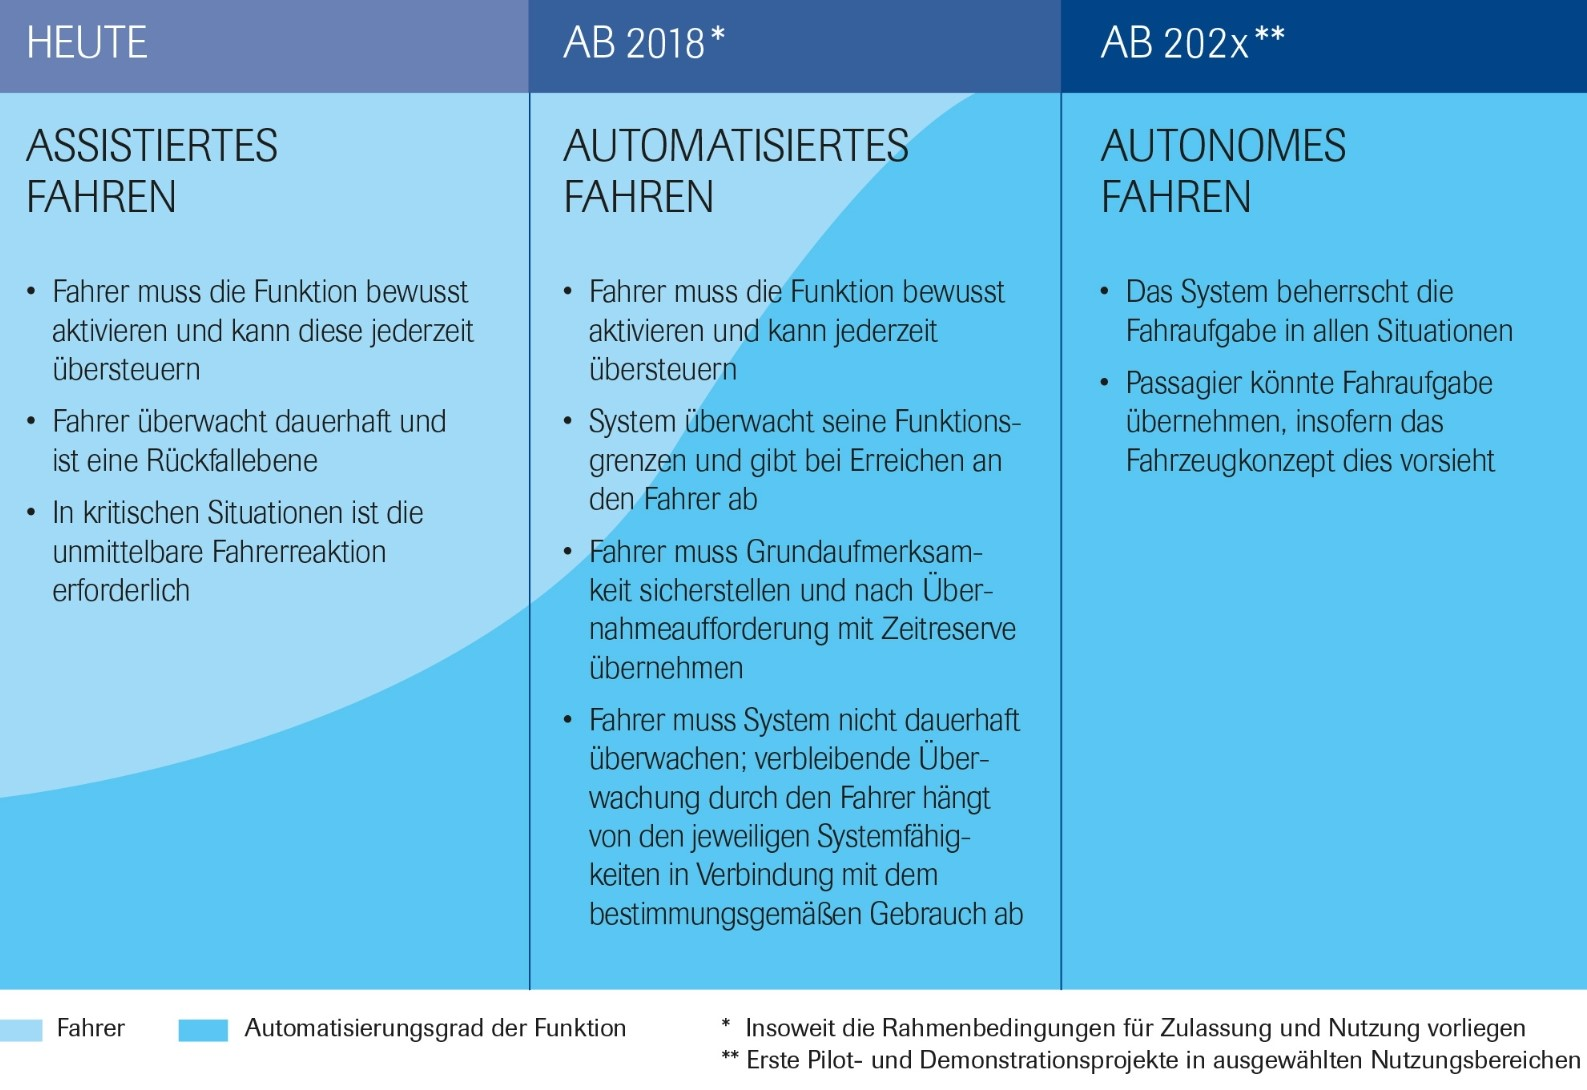
\includegraphics[width=11cm]{resources/zeitschiene-automatisierungsgrade.jpg}
\caption[Zeitschiene bei der Implementierung des automatisierten Fahrens]{Zeitschiene bei der Implementierung des automatisierten Fahrens~\cite{vda}}
\label{figure:ZeitschieneAutomatisierungsgrade}
\end{figure}

Die höchsten Automatisierungsgrade für das automatisierte Fahren, das \textit{vollautomatisierte} und das \textit{fahrerlose} Fahren, stehen also unmittelbar
vor der Einführung für den Testbetrieb, wobei dieser Trend weltweit zu beobachten ist.
Mit ihrem Papier~\cite{ek} hat die Ethikkommision die grundsätzlichen \glqq Leitplanken\grqq\ festgelegt, die bei der Implementierung des automatisierten Fahrens
beachtet werden sollten. Diese sind zu einem großen Teil unmittelbar einleuchtend, und als ein Angehöriger unseres westlichen Kulturkreises ist man grundsätzlich
intuitiv geneigt, ihnen vorbehaltlos zuzustimmen. Die Bundesregierung fasst in ihrem Maßnahmenplan~\cite{bmvi5} die Herausforderungen wie folgt zusammen:

\begin{quote}
\glqq
Die Zulassung automatisierter und vernetzter Fahrsysteme ist unter Berücksichtigung von Sicherheit, menschlicher Würde, persönlicher Entscheidungsfreiheit und Datenautonomie ethisch verantwortbar und kann gesellschaftlich und ethisch geboten sein, wenn damit vorhandene Potenziale der Schadensminimierung genutzt werden können. Der Schutz von Menschen muss Vorrang vor allen anderen Nützlichkeitserwägungen haben.\grqq\mbox{~\cite[S. 3]{bmvi5}}
\end{quote}

Es gibt jedoch zwei Problembereiche, die noch weitgehender diskutiert werden müssen: Der Ausschluss der totalen Überwachung und die 
Entscheidungsfähigkeit von Algorithmen in dilemmatischen Situationen.\\

Welche Daten der einzelne Fahrer der öffentlichen Hand oder seinen Vertragspartnern zur Verfügung stellen möchte, liegt grundsätzlich in dessen eigenem
Ermessen. Zumindest für das vollautomatisierte Fahren ist aber ein gewisses Mindestmaß an permanentem Datenaustausch unabdingbar. So werden 
Fahrzeugpositionen und damit auch die der Fahrer und Passagiere trotz Pseudonymisierung ähnlich wie derzeit schon bei der Mobilfunkortung nachvollziehbar 
und beispielsweise für Strafverfolgungsbehörden verfügbar sein. Ob dies gesellschaftlich vertretbar ist, muss in einem breiten Diskurs geklärt werden.  
Ein Blick nach China, wo derzeit ein IT-basiertes Punktesystem zur totalen Sozialkontrolle der Bürger etabliert wird~\cite{df}, zeigt, dass der noch akzeptable 
Grad sozialer Kontrolle je nach Kulturkreis offenbar sehr unterschiedlich ausgeprägt ist.\\

Die zweite ungeklärte Frage ist, inwieweit \glqq Moral\grqq\ bzw. \glqq Ethik\grqq\ grundsätzlich in Algorithmen implementierbar ist. Es macht eben einen grundlegenden
Unterschied, ob ein Unfallverursacher vor Gericht seine Entscheidung verantworten muss, in einem konkreten Fall den möglichen Tod oder die Verletzung eines älteren Rollstuhlfahrers gegenüber einer Gruppe von Kindern in Kauf genommen zu haben, oder ob ihm ein Algorithmus diese Entscheidung abnimmt. Wäre dies in der Software 
implementiert - einmal ganz abgesehen von den technischen Problemen - würde eben doch eine automatisierte Qualifizierung von Menschen stattfinden, die ganz 
klar der neunten Forderung der Ethik-Kommission widerspräche. Der Philosoph Richard D. Precht hat in einem nicht ganz von Polemik freien Artikel im \textit{Spiegel}
~\cite{pr} den Sachverhalt auf den folgenden Punkt gebracht:

\begin{quote}
\glqq
Dass der Code für jedes Problem eine Lösung haben soll, macht ihn nicht moralisch besser, sondern schlechter. Denn wem würde man eher verzeihen? Dem Fahrer,
der in seiner Not, um drei alte Damen zu schützen, versehentlich ein Kind überfährt? Oder einem bewusst einprogrammierten Ablauf, der den Damen einen
geringeren Lebenswert als dem Kind zuspricht, sich allerdings korrigiert, wenn er erkennt, dass das Kind, an äußeren Zeichen ablesbar, höchstwahrscheinlich
Leukämie hat?\grqq\mbox{~\cite[S. 79]{pr}}
\end{quote}

\noindent Precht plädiert daher für eine streng regelbasierte Lösung des Problems:

\begin{quote}
\glqq
Die erste Regel dürfte sein, den Insassen zu schützen. Wer steigt schon in ein Fahrzeug, das einen im Zweifelsfall opfert? Zweitens nach rechts ausweichen; drittens,
wenn das nicht geht, nach links. Das Fahrzeug muss dafür keine Gesichter erkennen, lediglich Menschen von Gegenständen unterscheiden. Mag sein, dass das Auto
dadurch vielleicht einmal die \glq falsche\grq\ Entscheidung trifft. Doch ist das nicht hundertmal besser, als ein programmiertes Abschätzen menschlichen Lebenswerts?\grqq\mbox{~\cite[S. 79]{pr}}
\end{quote}

\noindent Die Zukunft wird zeigen, wie wir mit diesem grundsätzlichen Problem umgehen.

\newpage

\cleardoublepage

\begin{thebibliography}{99}
\addcontentsline{toc}{section}{Literatur}

\bibitem{bt} Bluetooth Special Interest Group, Inc., Stand Januar 2019\\ \url{https://www.bluetooth.com/}

\bibitem{ek} Ethik-Kommission, eigesetzt durch das Bundesministerium für Verkehr und digitale Infrastruktur, Automatisiertes und
Vernetztes Fahren, 2017

\bibitem{epic} Electronic Privacy Information Center (EPIC), Automobile Event Data Recorders (Black Boxes) and Privacy,
\url{https://epic.org/privacy/edrs/}, \\Stand Januar 2019

\bibitem{bmjv} Bundesministerium der Justiz und für Verbraucherschutz (BMJV), Bundesamt der Justiz, Verordnung über die Zulassung von Personen zum Straßenverkehr, 
\url{http://www.gesetze-im-internet.de/fev_2010/}, Stand Januar 2019

\bibitem{bmvi1} Bundesministerium für Verkehr und digitale Infrastruktur (BMVI), Pressemitteilung 157/2016: Auftaktsitzung der Ethik-Kommission zum automatisierten Fahren,
\url{https://www.bmvi.de/SharedDocs/DE/Pressemitteilungen/2016/157-dobrindt-ethikkommission.html}, Stand Januar 2019

\bibitem{bmvi2} BMVI, Bericht zum Stand der Umsetzung der Strategie automatisiertes und vernetztes Fahren,
November 2017, \url{https://www.bmvi.de/SharedDocs/DE/Publikationen/DG/bericht-avf.html}, Stand Januar 2019

\bibitem{bmvi3} BMVI, Die mobile Zukunft beginnt jetzt! Wie automatisiertes und vernetztes Fahren den Verkehr revolutioniert,
November 2017, \url{https://www.bmvi.de/SharedDocs/DE/Publikationen/DG/automatisiertes-fahren.html}, Stand Januar 2019

\bibitem{bmvi4} BMVI, \glqq Eigentumsordnung\grqq\ für Mobilitätsdaten? Eine Studie aus technischer, ökonomischer und rechtlicher Perspektive,
August 2017, \url{https://www.bmvi.de/SharedDocs/DE/Publikationen/DG/eigentumsordnung-mobilitaetsdaten.html}, Stand Januar 2019

\bibitem{bmvi5} BMVI, Maßnahmenplan der Bundesregierung zum Bericht der Ethik-Kommission Automatisiertes und Vernetztes Fahren (Ethik-Regeln für
Fahrcomputer), September 2017, \url{https://www.bmvi.de/SharedDocs/DE/Publikationen/DG/massnahmenplan-zum-bericht-der-ethikkommission-avf.html}, 
Stand Januar 2019

\bibitem{df} Deutschlandfunk, Sozialkredit-System, China auf dem Weg in die IT-Diktatur, 09.09.2017, \url{https://www.deutschlandfunk.de/sozialkredit-system-china-auf-dem-weg-in-die-it-diktatur.724.de.html?dram:article_id=395440}, Stand Januar 2019

\bibitem{ho} G. Hornung, Verfügungsrechte an fahrzeugbezogenen Daten, in \textit{Datenschutz und Datensicherheit 2015}, \mbox{S. 359--366}

\bibitem{zeit1} D.\,H. Lamparter, Wer hat das Kommando?, in \textit{Die Zeit Nr. 9/2015}, \\
\url{https://www.zeit.de/2015/09/autonomes-fahren-assistenzsystem-autotechnik/komplettansicht}, Stand Januar 2019

\bibitem{pr} R.\,D. Precht, Maschinen ohne Moral, in \textit{Der Spiegel Nr. 48/2018} vom 24.11.2018, \mbox{S. 78--79},
\url{http://www.spiegel.de/plus/richard-david-precht-vom-irrsinn-maschinen-ethik-einzuprogrammieren-a-00000000-0002-0001-0000-000160960485}, Stand Januar 2019

\bibitem{dot} U.\,S. Department of Transportation (DOT), Preparing for the Future of Transportation: Automated Vehicle 3.0, 2018,
\url{https://www.transportation.gov/av}, Stand Januar 2019

\bibitem{vda} Verband der Automobilindustrie e.\,V. (VDA), \url{https://www.vda.de/de.html}, Stand Januar 2019

\bibitem{wi} Wikipedia, \url{https://de.wikipedia.org}, Stand Januar 2019

\end{thebibliography}

\newpage


\end{document}